221. Пусть $BC=1,\ AD=3.$\\
1) \begin{figure}[ht!]
\center{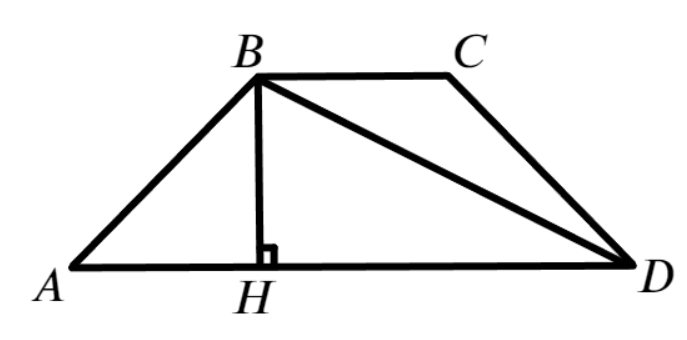
\includegraphics[scale=0.35]{g8-221-1.png}}
\end{figure}\\
Опустим высоту $BH,$ тогда, так как трапеция равнобедренная, $AH=\cfrac{3-1}{2}=1.$ Поэтому $HD=3-1=2$ и по теореме Пифагора $BD=\sqrt{1^2+2^2}=\sqrt{5}<3,$ значит первое утверждение неверно.\\
2) \begin{figure}[ht!]
\center{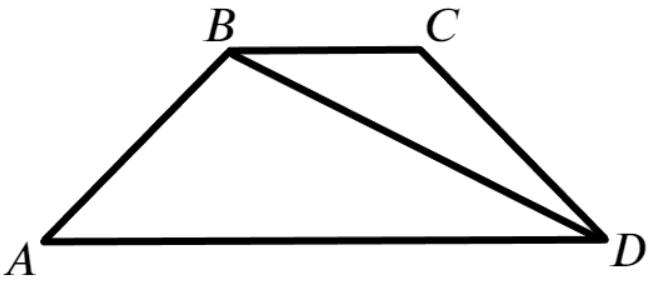
\includegraphics[scale=0.35]{g8-221-2.png}}
\end{figure}\\
Если $BD>3,$ то $BD>AD,$ значит $\angle A>\angle ABD.$ Если $\angle A\leqslant 45^\circ,$ то $\angle ABD<45^\circ$ и $\angle ADB=180^\circ-\angle A-\angle ABD>90^\circ,$ что невозможно. Значит, $\angle A>45^\circ$ и второе утверждение верно.\\
3) \begin{figure}[ht!]
\center{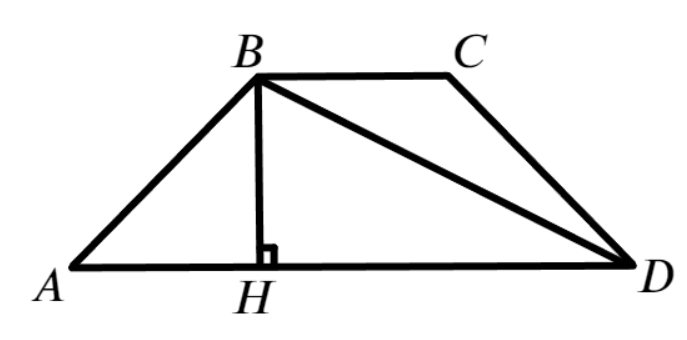
\includegraphics[scale=0.35]{g8-221-1.png}}
\end{figure}\\
Опустим высоту $BH,$ тогда, так как трапеция равнобедренная, $AH=\cfrac{3-1}{2}=1$ и по теореме Пифагора $BH=\sqrt{2^2-1^2}=\sqrt{3}.$ Таким образом, $S=\sqrt{3}\cdot\cfrac{1+3}{2}=2\sqrt{3}<4.$ Значит, третье утверждение неверно.\\
4) \begin{figure}[ht!]
\center{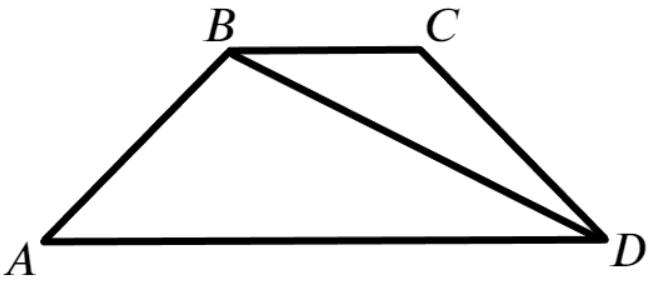
\includegraphics[scale=0.35]{g8-221-2.png}}
\end{figure}\\
Если $S=BH\cdot\cfrac{1+3}{2}=2BH=1,$ то $BH=\cfrac{1}{2}.$ Тогда по теореме Пифагора $BD=\sqrt{\cfrac{1}{4}+4}=\cfrac{\sqrt{17}}{2}$ и $AB=CD=\sqrt{\cfrac{1}{4}+1}=\cfrac{\sqrt{5}}{2}.$ Окружность, описанная вокруг трапеции $ABCD,$ является также описанной окружностью треугольника $BCD.$ Найдём его площадь двумя способами. С одной стороны, $S_{\Delta BCD}=\cfrac{1}{2}\cdot\cfrac{1}{2}\cdot1=\cfrac{1}{4}.$ С другой стороны, $S_{\Delta BCD}=\cfrac{1\cdot\cfrac{\sqrt{5}}{2}\cdot\cfrac{\sqrt{17}}{2}}{4R}=\cfrac{\sqrt{85}}{16R},$ откуда $\cfrac{1}{4}=\cfrac{\sqrt{85}}{16R},\ R=\cfrac{\sqrt{85}}{4}>1,$ значит четвёртое утверждение верно.\\
